% ============================================================================
% Build: make qdd-liquid-paper-pdf   (tectonic main.tex)
% Figures and numbers.json: make qdd-liquid-paper  (paper/figures.py)
% Every number here is printed by a script in qdd-liquid/; see the README there.
%
% FRAMING NOTE: nothing in this paper has been built or measured. Cooling a
% winding from inside a hollow conductor is long-established; no novelty is
% claimed for it. Do not add language implying hardware results.
% ============================================================================
\documentclass[11pt]{article}

\usepackage[margin=1.1in]{geometry}
\usepackage[T1]{fontenc}
\usepackage[utf8]{inputenc}
\usepackage{lmodern}
\usepackage{microtype}
\usepackage{amsmath}
\usepackage{booktabs}
\usepackage{graphicx}
\usepackage{siunitx}
\usepackage{wasysym}
\usepackage[numbers,sort&compress]{natbib}
\usepackage[hidelinks]{hyperref}

\sisetup{detect-all}
\DeclareSIUnit\rms{rms}
\newcommand{\code}[1]{\texttt{\small #1}}
\newcommand{\Amm}{\si{A\per\milli\metre\squared}}
\newcommand{\Nm}{\si{N.m}}

\title{\textbf{Cooling a Quasi-Direct-Drive Joint Motor from Inside the Copper:\\
A Simulation-Only Design Study}}
\author{Dan Newcome\\[2pt]
  \small punkfab\\
  \small\url{https://github.com/punkfab/robot-actuators}}
\date{October 2026}

\begin{document}
\maketitle

\begin{abstract}
Quasi-direct-drive (QDD) robot joints trade gear ratio for transparency, and
their continuous torque is set by how much winding heat the housing can shed.
We test one hypothesis: that drive electronics are now efficient enough at
high current that heat is the remaining limit, so a joint motor should be cooled
directly, run hard, and geared less. The design studied is a
\diameter\SI{120}{mm}, 24-slot, 22-pole motor whose coils are hollow rectangular
copper carrying dielectric oil in the bore, inside an outer jacket fed with the
coldest coolant. It is evaluated with a first-order loss and hydraulic model, a
nonlinear two-dimensional magnetostatic field solution written for the study,
a lumped thermal model of the jacket-only alternative, and a parametric CAD
assembly with interference checks, all driven by one design record.
\emph{Nothing has been built or measured.} In simulation the motor gives
\SI{16.6}{\Nm} continuously for \SI{850}{W} of heat with the copper at
\SI{126}{\celsius}, and \SI{21.3}{\Nm} at the limit of a
\SI{3}{L\per\minute} pump, against about \SI{5}{\Nm} for the same iron cooled
by air. Three results ran against the hypothesis. The saturation limit
first assumed was too pessimistic, by a quarter to a third of the torque. Trading copper for iron at
fixed size does not raise torque at a given heat: eleven geometry variants land
within about \SI{10}{\percent} of each other. And a much simpler motor, with
solid conductors and only the jacket, reaches about \SI{70}{\percent} of the
hollow design's torque, so it is the one to build first. A
\num{3}:\num{1} reduction then matches a commercial \num{9}:\num{1} actuator's
continuous torque with a ninth of the reflected inertia, and spends about five
times the power holding the same load. The models and CAD were written by an AI coding agent under the
author's direction; we describe that workflow and the modelling errors that
cross-checks between the models exposed. No new cooling method is claimed. The
contributions are the design, its comparison with the jacket-only motor, and
the open code.
\end{abstract}

% ============================================================================
\section{Introduction}
\label{sec:intro}

The proprioceptive, or quasi-direct-drive, actuator pairs a large-diameter
torque motor with a single low-ratio gear stage, so that the joint is
backdrivable, its reflected inertia is small, and motor current is a usable
measure of output torque~\cite{wensing2017,seok2015,katz2018}. The price is
that torque comes from current instead of from gearing. Copper loss rises with
the square of torque, and the continuous rating of such a joint is a thermal
figure: what the winding can lose through the slot insulation, the iron, the
housing and whatever the housing is bolted to.

This study tests a design hypothesis: high-current solid-state drives are now
efficient enough that heat, not the drive, limits a joint motor, so the
conductors should be cooled directly with liquid, the hot machine isolated
from its surroundings by an outer jacket, the copper run at high current
density and temperature, and the gear ratio reduced.

The contributions are:

\begin{enumerate}
\item a hollow-conductor, oil-cooled motor design in the envelope of a
  commercial QDD actuator, evaluated by loss, hydraulic and nonlinear field
  models and drawn as a checked CAD assembly;
\item a comparison, on the same iron, with a jacket-only motor using solid
  conductors, and the consequences of both for gear ratio and holding power;
\item the open models and solver, and a description of the agent-assisted
  workflow that produced them, including the errors found by cross-checking
  (Section~\ref{sec:process}).
\end{enumerate}

\paragraph{Scope.} The study is simulation only: nothing has been built or
measured. Cooling a winding by passing coolant through hollow conductors is
decades old in large machines and has been demonstrated in small ones
(Section~\ref{sec:related}); no novelty is claimed for the method. Every
thermal coefficient is a handbook value or a stated assumption, and
Section~\ref{sec:limits} lists what the models leave out.

% ============================================================================
\section{Related work}
\label{sec:related}

\paragraph{Quasi-direct-drive actuators.} The design principles are those of
the MIT Cheetah: a high-torque-density motor, a low gear ratio, and torque
control through motor current~\cite{seok2015,wensing2017}, later made low-cost
and modular by \citet{katz2018}. \citet{seok2015} report that
\SI{76}{\percent} of their robot's energy in trotting is motor heat, which is
the loss this study is about.

\paragraph{Liquid cooling of robot actuators.} Cooling a robot's motors with
liquid is established. \citet{urata2010} combined forced liquid cooling with estimation of the
motor's internal temperature in a high-power humanoid leg.
\citet{paine2015} retrofitted liquid cooling to an off-the-shelf motor and
measured 2.58 times the continuous torque, and \citet{kim2018} and
\citet{zhu2019} built and modelled liquid-cooled actuators. \citet{mazumdar2016} report \SI{50}{\percent} more heat transfer from a
redesigned motor housing, and \SI{107}{\percent} more with pumped water.
\citet{kozuki2016} used a humanoid's skeleton to release heat by latent heat,
and \citet{li2026} cool humanoid joint motors by evaporation from
phase-change hydrogels. Closest to the winding, \citet{zhu2021} immersed the
coils of a legged-robot motor directly in coolant, built and tested it, and
report a thermal resistance 3.7 times better than liquid cooling and 10 times
better than forced air. That last work is the nearest to ours: it
already brings coolant into contact with the winding of a legged-robot motor.

\paragraph{Coolant inside the conductor.} Hollow stator conductors carrying
water are long-standing practice in large turbo-generators~\cite{bauer2021,
svoboda2004}. In smaller machines, \citet{lindh2016,lindh2017} cooled the
tooth coils of an axial-flux traction machine with oil or water in a stainless
tube wrapped in Litz wire and compared it with water jackets;
\citet{schiefer2015} placed water channels in the unused slot space of a
concentrated winding; \citet{wohlers2018} studied direct liquid cooling of
tooth-coil windings; and \citet{wu2020,wu2021} designed additively manufactured hollow
conductors for aircraft machines. \citet{geelen2024} is a simulation study of
water-cooled hollow conductors in coreless linear motors. Reviews of
machine cooling are given by \citet{gai2019} and \citet{yang2017}, and the
sizing relations we use are standard~\cite{pyrhonen2013}.

\paragraph{Where this study sits.} We found no published robot joint motor
with coolant inside the winding conductor. Our search covered the indexed
English-language literature and did not cover patents or work in other
languages, so we do not claim there is none. What this study adds is narrow:
the hollow-conductor scheme sized for a QDD joint envelope, the comparison
with the jacket-only motor on the same iron, and the consequence for gear
ratio.

% ============================================================================
\section{Concept}
\label{sec:concept}

\begin{figure}[t]
\centering
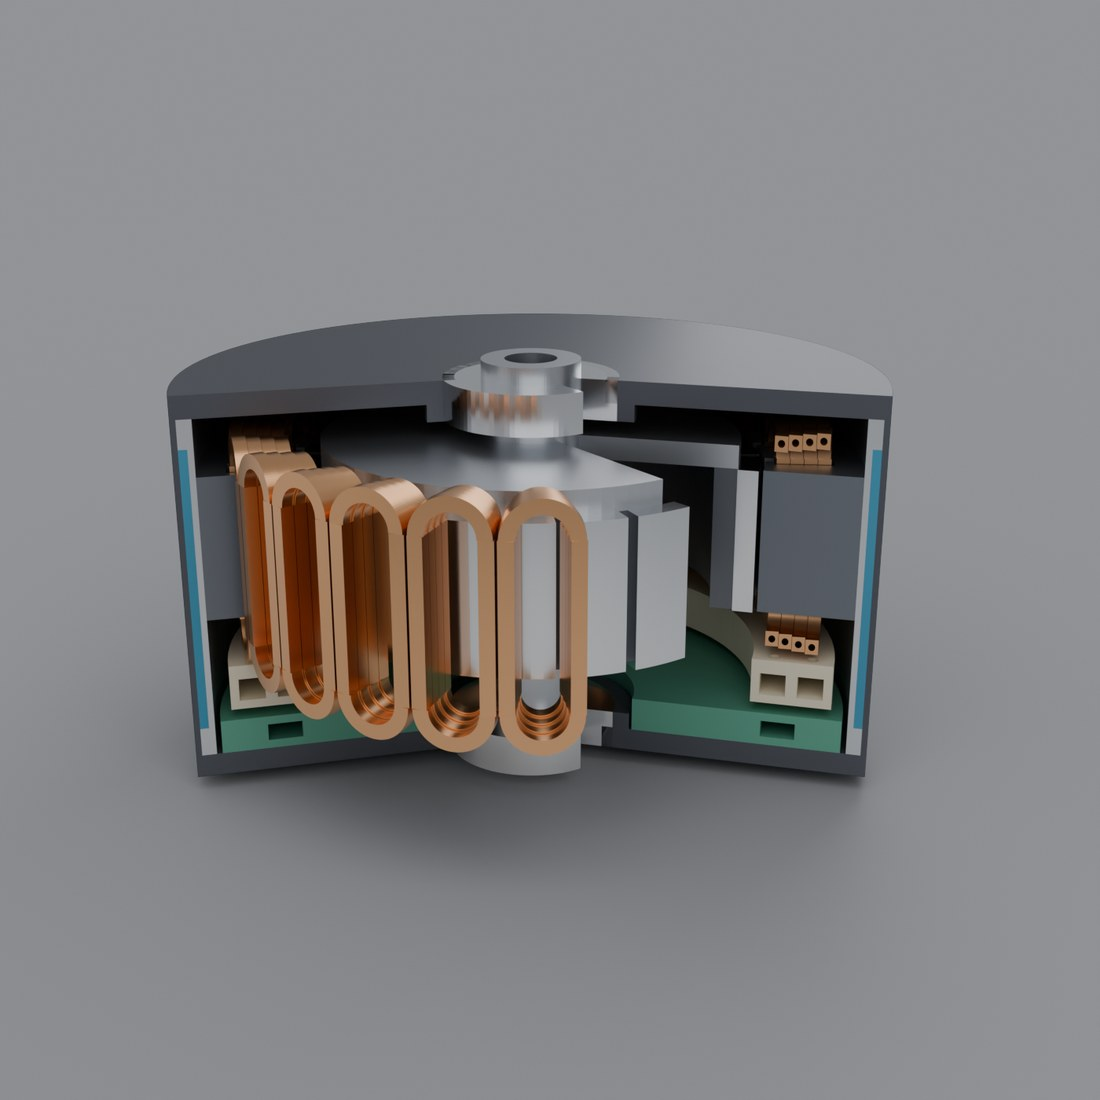
\includegraphics[width=0.49\linewidth]{figures/cutaway.jpg}\hfill
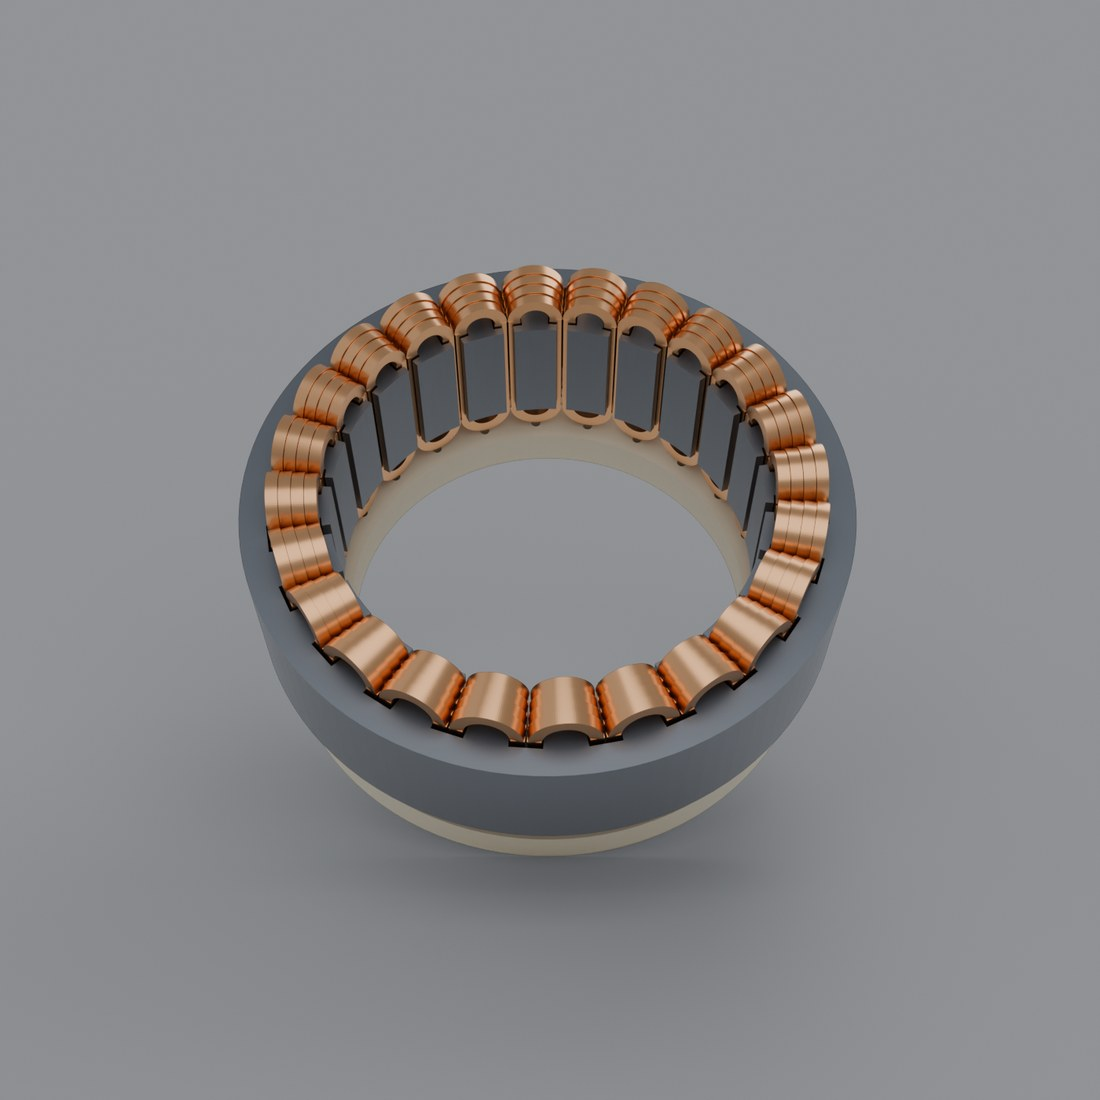
\includegraphics[width=0.49\linewidth]{figures/stator.jpg}
\caption{The shallow-slot design, rendered from the CAD assembly. Left: cutaway
with the hollow conductors in section, the magnets, the coolant (blue) in the
jacket channel, the manifold ring and the drive plate. Right: the wound stator
with its 24 single-column coils.}
\label{fig:render}
\end{figure}

The motor (Figure~\ref{fig:render}) has these features.

\begin{itemize}
\item \textbf{Hollow copper conductors.} Coolant flows in the bore of every
  turn, so heat leaves from inside the copper instead of crossing insulation,
  iron and a housing.
\item \textbf{Few turns of large conductor.} A low-voltage, high-current
  machine, with one coil per tooth (24 slots, 22 poles).
\item \textbf{Dielectric oil.} It can touch live copper, so the coils are
  electrically in series and hydraulically in parallel with no insulating
  breaks.
\item \textbf{The drive on the motor,} with its cold plate on the same loop.
\item \textbf{An outer jacket fed first.} The flow order is
  radiator $\rightarrow$ drive cold plate $\rightarrow$ outer jacket
  $\rightarrow$ conductor bores $\rightarrow$ radiator. The coldest fluid
  lines the outside of the machine before it reaches the heat source, in the
  way a regeneratively cooled rocket nozzle is lined by its
  propellant~\cite{sutton2017}.
\item \textbf{Stator outside,} pressed into the jacket, with the rotor inside
  and a \diameter\SI{64}{mm} free bore.
\end{itemize}

The envelope is that of the RobStride RS04~\cite{robstride-rs04}, a
\diameter\SI{120}{mm} actuator with a \num{9}:\num{1} reduction rated at
\SI{35}{\Nm} continuous (on a $220\times\SI{200}{mm}$ heat sink) and
\SI{120}{\Nm} peak, which serves as the reference
throughout.

% ============================================================================
\section{Models}
\label{sec:models}

All four models read one frozen design record (\code{design.Design}), so the
field solver, the loss model and the CAD cannot disagree about a dimension.

\subsection{Sizing: losses, hydraulics, drive}
\label{sec:sizing}

Unsaturated torque is
\begin{equation}
T = 3\,k_w N_{ph} B_1 r_g L \,\hat{I},
\label{eq:torque}
\end{equation}
with winding factor $k_w = 0.95$, $N_{ph}$ series turns per phase, $B_1$ the
peak of the air-gap field's working harmonic, $r_g$ the gap radius, $L$ the
stack length and $\hat I$ the peak phase current. Copper loss is
$P_{cu} = \rho(\theta) J^2 V_{cu}$ with
$\rho(\theta)=\rho_{20}\,[1+\alpha(\theta-20)]$, $\alpha=\SI{0.00393}{\per\kelvin}$,
evaluated at the mean copper temperature, which the model solves for.

Each coil is one hydraulic path. For a pressure $\Delta p$ across it the bore
velocity $v$ follows from $\Delta p = f\,(\ell/d)\,\rho v^2/2$, with $f=64/Re$
in laminar flow blended to the Blasius form above $Re=2300$, and the film
coefficient from $Nu=4.36$ blended to the Dittus--Boelter
correlation~\cite{bergman2011}. The
hottest copper is at the coil outlet:
\begin{equation}
\theta_{max} = \theta_{in} + \frac{P_{drv}+P_{fe}}{\dot m c_p}
  + \frac{P_{cu}}{\dot m c_p}
  + \frac{P_{cu}/N_s}{h\,\pi d\,\ell},
\label{eq:tmax}
\end{equation}
where the second term is the rise across the drive plate and jacket, which the
coolant passes first. Drive loss is conduction in the switches and leads plus
switching, $P_{drv}=3I^2(R_{ds}+R_{lead}) + 3\,(0.9V_{bus})\,I\,t_{sw}f_{sw}$,
with $R_{ds}=\SI{0.5}{m\ohm}$ per switch position, $R_{lead}=\SI{0.2}{m\ohm}$,
\SI{48}{V}, \SI{40}{kHz} and \SI{20}{ns}, all assumed. Pump power is
$\Delta p\,Q/\eta$ with $\eta=0.4$.

Two choices in this model matter to the results. The pump pressure at each
operating point is the one that gives the \emph{least total heat} (more flow
costs pump power but cools the copper and lowers its resistance), and total
flow is capped at \SI{3}{L\per\minute}, our assumption for what a joint-sized
pump and hoses carry. The continuous limit is the current at which the hottest
copper reaches \SI{200}{\celsius} under that cap. The oil is a
polyalphaolefin-class dielectric with handbook properties
(at \SI{66}{\celsius}: \SI{785}{kg\per\metre\cubed},
\SI{2190}{J\per\kg\per\kelvin}, \SI{0.138}{W\per\metre\per\kelvin},
\SI{2.5}{mPa.s}), entering at \SI{60}{\celsius}.

\subsection{Field solution}
\label{sec:fea}

Equation~\eqref{eq:torque} needs $B_1$ and says nothing about saturation, so the
sizing model first carried an assumed air-gap field and an assumed saturation
knee (an air-gap shear of \SI{90}{kPa}). To replace both we wrote a
two-dimensional magnetostatic solver for the cross-section. It solves
\begin{equation}
\nabla\cdot\bigl(\nu(|\mathbf B|^2)\,\nabla A_z\bigr) = -J_z - \nabla\times(\nu\,\mathbf B_r)\cdot\hat z
\end{equation}
for the axial vector potential on linear triangles generated by
Gmsh~\cite{geuzaine2009}, with $A_z=0$ on the outer boundary. The iron's
reluctivity follows Brauer's fit~\cite{brauer1975},
$\nu = k_1 e^{k_2 B^2} + k_3$ with $(k_1,k_2,k_3)=(3.8,\,2.17,\,396.2)$,
a generic non-oriented electrical steel, continued at the slope of free space
beyond the flux density where the fit becomes that steep (about
\SI{2.07}{T}). Newton iteration with backtracking uses the element tangent
\begin{equation}
K_e = \Delta_e\,\nu\,G^\top G + 2\Delta_e\,\frac{d\nu}{dB^2}\,
      (G^\top\nabla A)(G^\top\nabla A)^\top ,
\end{equation}
where $G$ holds the shape-function gradients and $\Delta_e$ is the element
area. Magnets have $B_r=\SI{1.17}{T}$, $\mu_r=1.05$ and cover
\SI{85}{\percent} of the pole pitch. Torque is Arkkio's integral over the
air-gap elements~\cite{arkkio1987},
$T = \tfrac{L}{\mu_0 (r_o-r_i)}\int r B_r B_\theta\,dS$. The current angle is
chosen by a sweep at each end of the current range.

Two checks on the solver, both on the final design:
\begin{itemize}
\item \emph{Mesh refinement.} At \SI{32.5}{\Amm}, torque is \num{16.56},
  \num{16.58} and \SI{16.55}{\Nm} on \num{17986}, \num{30764} and \num{76023}
  triangles: a spread of \SI{0.2}{\percent}. The middle mesh is used.
\item \emph{Closed form.} At \SI{3}{\Amm}, well below saturation, the solver
  gives \SI{1.611}{\Nm}. Equation~\eqref{eq:torque} with the solver's own
  no-load $B_1=\SI{1.053}{T}$ gives \SI{1.644}{\Nm}, \SI{2}{\percent} higher.
\end{itemize}
Neither is a validation against a measured machine or an independent code, and
the solver is two-dimensional at one rotor position (Section~\ref{sec:limits}).

\subsection{Jacket-only thermal path}
\label{sec:jacketmodel}

For the alternative with solid conductors, all copper heat crosses, per tooth:
conductor insulation and slot liner, tooth, yoke, the press fit to the jacket,
and the coolant film. We model that as five resistances in series per metre of
stack, with a liner conductivity of \SI{0.2}{W\per\metre\per\kelvin}
(unpotted), in-plane lamination conductivity
\SI{25}{W\per\metre\per\kelvin}, a fit conductance of
\SI{2000}{W\per\metre\squared\per\kelvin} and a film coefficient of
\SI{1500}{W\per\metre\squared\per\kelvin}. All four are assumed. End-turn heat
is taken to conduct along the copper into the slot. This is a lumped model,
not a thermal field solution.

\subsection{CAD as a check}
\label{sec:cad}

A build123d~\cite{build123d} script generates thirteen part types from the
same design record: stator core, 24 coils, a two-piece jacket with its annular
channel, rotor yoke, 22 magnets, rotor carrier, a manifold ring with supply
and return plenums, drive cold plate, two end caps, bearings and shaft. It
exports a STEP assembly and computes the shared volume of thirteen part pairs.
Its purpose here is to test whether the conductor the loss model assumes can
be placed in the slot the field model assumes. Each turn is drawn as a closed
racetrack; crossovers, leads, fasteners, seals and bus bars are not drawn.

% ============================================================================
\section{Results}
\label{sec:results}

\subsection{The assumed saturation limit was wrong}

On the first geometry (wedge slots \SI{14}{mm} deep, half the slot pitch), the
field solution gives more torque than the assumed knee at every current
(Table~\ref{tab:knee}). The no-load air-gap field is \SI{1.04}{T} against the
\SI{0.83}{T} assumed, and saturation is far more gradual: torque per amp is
still \SI{92}{\percent} of its unsaturated value at \SI{26}{\Amm}, where the
assumed knee had the motor close to its ceiling.

\begin{table}[h]
\centering
\begin{tabular}{rrrrr}
\toprule
current density & field solution & torque per amp & assumed knee & total heat\\
\midrule
\SI{14}{\Amm} & \SI{8.5}{\Nm} & \SI{98}{\percent} & \SI{6.8}{\Nm} & \SI{188}{W}\\
\SI{26}{\Amm} & \SI{14.8}{\Nm} & \SI{92}{\percent} & \SI{10.7}{\Nm} & \SI{674}{W}\\
\SI{33}{\Amm} & \SI{17.5}{\Nm} & \SI{86}{\percent} & \SI{12.2}{\Nm} & \SI{1135}{W}\\
\SI{42}{\Amm} & \SI{20.2}{\Nm} & \SI{77}{\percent} & \SI{13.5}{\Nm} & \SI{2.0}{kW}\\
\SI{100}{\Amm} & \SI{26.4}{\Nm} & \SI{43}{\percent} & \SI{16.6}{\Nm} & beyond the pump\\
\bottomrule
\end{tabular}
\caption{First geometry: the field solution against the saturation knee the
sizing model had assumed.}
\label{tab:knee}
\end{table}

In that geometry torque per amp is down \SI{20}{\percent} at \SI{39}{\Amm}
(\SI{19.3}{\Nm}) and the \SI{3}{L\per\minute} pump is exhausted at
\SI{49}{\Amm} (\SI{21.4}{\Nm}, about \SI{3}{kW}). Heat and saturation arrive
at nearly the same current. The premise that heat is \emph{the} limit
is therefore half right for this iron: remove the heat and the iron is next,
immediately.

\subsection{More iron in the same size does not help}

The natural response is to widen the teeth. Table~\ref{tab:variants} holds the
envelope at \diameter\SI{120}{mm} with a \SI{25}{mm} stack and trades copper
for iron.

\begin{table}[h]
\centering
\small
\begin{tabular}{lrrrrr}
\toprule
 & \multicolumn{3}{c}{torque (\si{\Nm}) at total heat} & cooling & $K_t$ down\\
variant & \SI{300}{W} & \SI{850}{W} & \SI{1500}{W} & limit & \SI{20}{\percent} at\\
\midrule
baseline: slots 50\% of pitch, \SI{14}{mm} deep & 10.5 & 15.9 & 18.8 & 21.4 & \SI{39}{\Amm}\\
slots 40\% & 9.7 & 15.4 & 18.8 & 22.3 & \SI{57}{\Amm}\\
slots 30\% & 8.5 & 13.7 & 17.0 & 20.6 & \SI{79}{\Amm}\\
slots \SI{10}{mm} deep (larger rotor) & 10.5 & 16.7 & 20.7 & 25.0 & \SI{65}{\Amm}\\
slots 40\%, \SI{10}{mm} deep & 9.6 & 15.5 & 19.6 & 24.5 & \SI{98}{\Amm}\\
slots 30\%, \SI{7}{mm} deep & 7.7 & 12.6 & 16.1 & 18.8 & over \SI{140}{\Amm}\\
magnets \SI{5}{mm} & 10.7 & 16.2 & 19.2 & 22.0 & \SI{40}{\Amm}\\
cobalt-iron laminations & 10.8 & 16.8 & 20.2 & 23.5 & \SI{46}{\Amm}\\
outrunner & 11.8 & 17.6 & 20.9 & 24.0 & \SI{36}{\Amm}\\
\bottomrule
\end{tabular}
\caption{Copper traded for iron at fixed envelope, idealised conductor fill.
The cooling-limit column is torque in \si{\Nm}; $K_t$ is torque per amp.
Nine of the eleven variants run are shown; the other two (a thicker yoke, and
an outrunner with narrow shallow slots) fall inside the same range.}
\label{tab:variants}
\end{table}

Wider teeth do push saturation out, a long way. They also remove copper, so
the same torque needs a higher current density and makes more heat. The two
effects nearly cancel: at \SI{850}{W} every variant but the most iron-rich is
within about \SI{10}{\percent} of the others. The one clear gain is a
shallower slot, which lets the rotor grow: \SI{+5}{\percent} at \SI{850}{W}
and \SI{+17}{\percent} at the cooling limit. An outrunner is worth about
\SI{11}{\percent}, not the factor of 1.5 the first-order model had suggested,
and cobalt-iron about \SI{6}{\percent}.

At this size the motor makes about \SI{16}{\Nm} for \SI{850}{W} whatever the
split between copper and iron. More torque at the same heat means more stack
length or more diameter: the trade is size for torque, not size for iron.

\subsection{The shallow-slot design}

\begin{table}[t]
\centering
\small
\begin{tabular}{ll}
\toprule
envelope & \diameter\SI{120}{mm} $\times$ \SI{68}{mm}, \SI{25}{mm} stack, \diameter\SI{64}{mm} free bore\\
slots / poles & 24 / 22, slots parallel-sided, \SI{5.8}{mm} wide, \SI{10}{mm} deep\\
coil & one per tooth, a single column of 4 turns\\
conductor & hollow rectangular copper, $2.4\times\SI{2.2}{mm}$, \diameter\SI{1.2}{mm} bore, \SI{4.1}{mm\squared}\\
no-load air-gap field & \SI{1.05}{T} (working harmonic, peak)\\
\midrule
continuous, \SI{850}{W} total heat & \SI{16.6}{\Nm} at \SI{132}{A} rms per phase (\SI{32.5}{\Amm})\\
heat at that point & copper \SI{793}{W}, drive and leads \SI{51}{W}, pump \SI{3}{W}\\
coolant & in \SI{60}{\celsius}, out \SI{71}{\celsius}, \SI{2.6}{L\per\minute}, \SI{0.28}{bar}, $Re\approx 610$\\
temperatures & skin \SI{61}{\celsius}, hottest copper \SI{126}{\celsius}, magnets about \SI{90}{\celsius}\\
cooling limit (\SI{3}{L\per\minute}) & \SI{21.3}{\Nm} at \SI{43}{\Amm}, about \SI{1.8}{kW}\\
torque per amp down \SI{20}{\percent} & at \SI{67}{\Amm} (\SI{28.6}{\Nm}), beyond the pump\\
motor mass & about \SI{1.7}{kg} (estimate, no gear stage)\\
\bottomrule
\end{tabular}
\caption{The shallow-slot design, as simulated.}
\label{tab:design}
\end{table}

\begin{figure}[t]
\centering
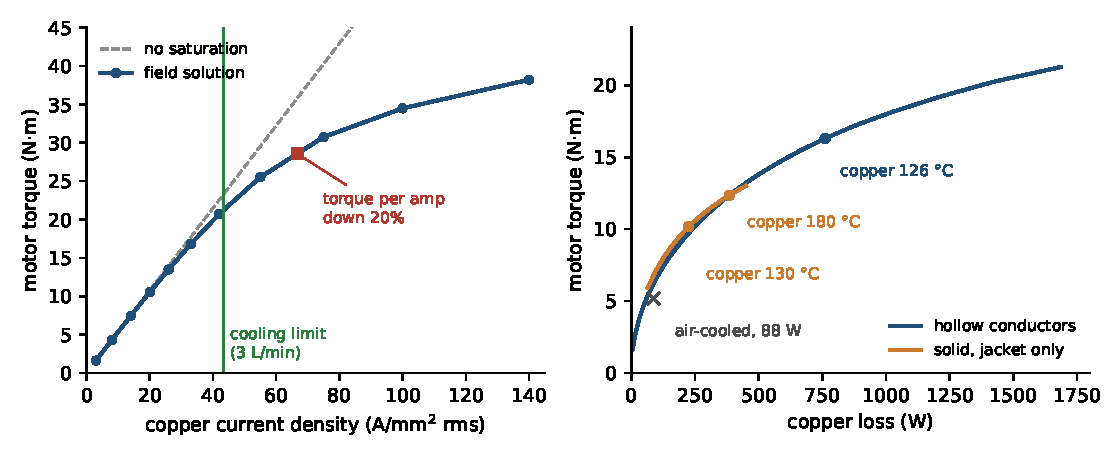
\includegraphics[width=\linewidth]{figures/torque.pdf}
\caption{Shallow-slot design. Left: field-solved torque against copper current
density. Right: torque against copper loss for hollow conductors and for solid
conductors with only the jacket; the curves end where each cooling scheme
does. The air-cooled point is the same iron with a conventional winding.}
\label{fig:torque}
\end{figure}

\begin{figure}[t]
\centering
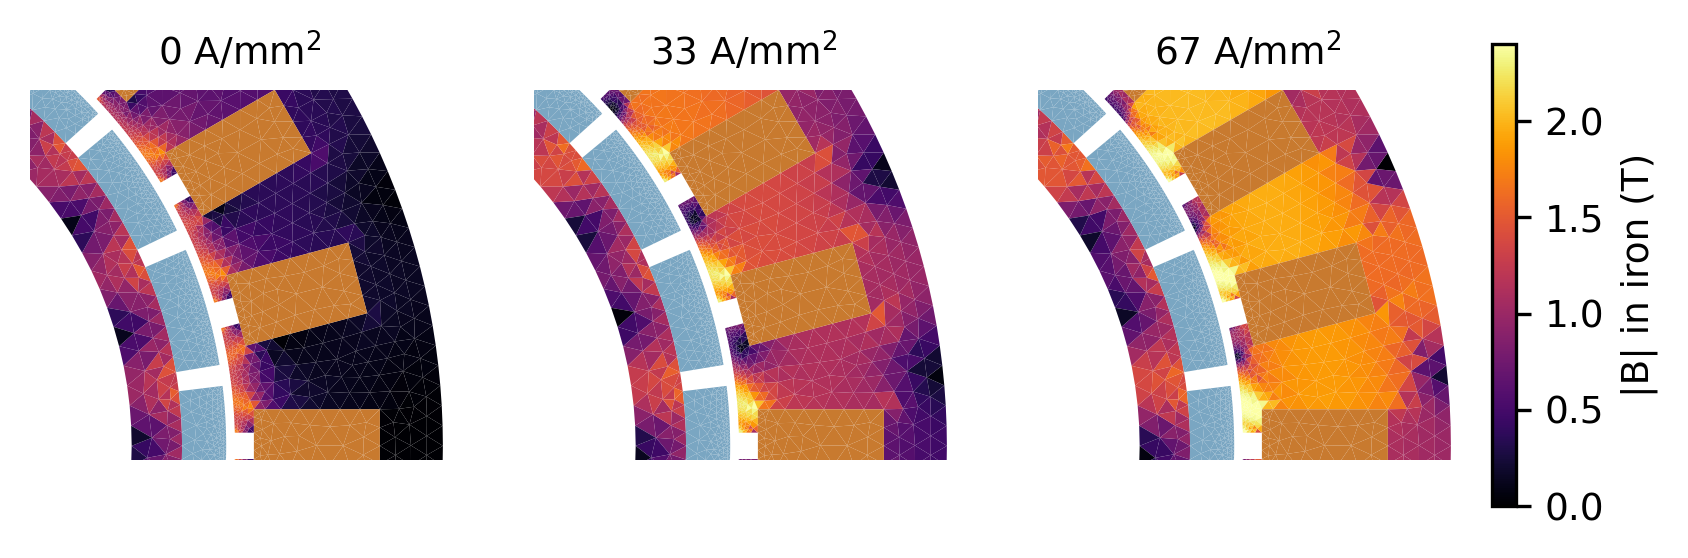
\includegraphics[width=\linewidth]{figures/field.png}
\caption{Flux density in the iron of the shallow-slot design at no current, at
the \SI{850}{W} point, and where torque per amp is down \SI{20}{\percent}.}
\label{fig:field}
\end{figure}

Table~\ref{tab:design} and Figures~\ref{fig:torque} and~\ref{fig:field} give
the design that follows from the variant study, now with a specific conductor
in parallel-sided slots. Here cooling is the limit again: the pump runs out at
\SI{43}{\Amm} with torque per amp still at \SI{92}{\percent}. The flow in the
bores is laminar, so the film coefficient is fixed by the bore diameter and
the limit is set by the coolant's temperature rise, which is why the flow cap
matters more than the pump pressure. The jacket does what it was drawn for:
the skin sits within about a degree of the coolant inlet at every operating
point. The same iron wound conventionally and limited to \SI{88}{W} of copper
loss gives about \SI{5}{\Nm}.

Among six conductor layouts compared, round capillary tube (an off-the-shelf
part) fills only \SI{39}{\percent} of the slot and gives \SI{12.8}{\Nm} at
\SI{850}{W}, a quarter less than the rectangular conductor, which is a custom
draw. Three or five turns per coil in slots \SI{8}{mm} or \SI{12}{mm} deep give
\SI{15.4}{\Nm} and \SI{16.9}{\Nm}.

\subsection{What the CAD caught}

\begin{itemize}
\item \emph{Coils sharing a slot collided.} At a conductor pitch of
  \SI{2.6}{mm} the two coil sides in one slot were \SI{0.2}{mm} apart and
  their end bends crossed as they left the slot. The pitch is now
  \SI{2.5}{mm}, \SI{0.4}{mm} apart, and all thirteen pair checks report no
  shared volume. The loss and field models were rerun with the new conductor.
\item \emph{The end bends are tight.} The bend radius on the conductor centre
  is \SIrange{4.2}{5.1}{mm} for a conductor \SI{2.4}{mm} wide: under twice its
  width, on a hollow section. Whether that can be formed without collapsing
  the bore is a question for a forming trial, and it is the first thing we
  would test.
\end{itemize}

\subsection{The simpler motor: solid conductors, jacket only}
\label{sec:jacket}

Filling in the bore gives \SI{28}{\percent} more copper and removes the
manifold, the custom conductor and the oil-to-copper joints. All heat then
leaves through the tooth. With coolant at \SI{60}{\celsius}:

\begin{table}[h]
\centering
\begin{tabular}{lrrr}
\toprule
 & torque & copper loss & hottest copper\\
\midrule
jacket only & \SI{9.6}{\Nm} & \SI{200}{W} & \SI{130}{\celsius}\\
jacket only & \SI{11.7}{\Nm} & \SI{343}{W} & \SI{180}{\celsius}\\
hollow conductors & \SI{16.6}{\Nm} & \SI{793}{W} & \SI{126}{\celsius}\\
hollow conductors, pump limit & \SI{21.3}{\Nm} & about \SI{1.7}{kW} & \SI{198}{\celsius}\\
\bottomrule
\end{tabular}
\caption{Jacket-only cooling against hollow conductors, same iron and slots.}
\label{tab:jacket}
\end{table}

The jacket alone gives about \SI{70}{\percent} of the hollow design's
\SI{850}{W} torque and \SI{55}{\percent} of its limit, with ordinary wire.
Figure~\ref{fig:torque} (right) shows why the comparison is close: per watt of
copper loss the two windings give nearly the same torque, and the hollow
conductor's advantage is only that its curve continues. It does this well
because each coil is a single column, so every conductor has a face on a tooth
wall. The slot liner is \SI{41}{\percent} of the thermal path, the coolant
film \SI{22}{\percent}, the press fit \SI{16}{\percent}, the tooth
\SI{15}{\percent} and the yoke \SI{7}{\percent}, so the result depends on how
the coil is seated: at \SI{180}{\celsius} copper, a loose coil with a
\SI{0.05}{mm} air gap gives \SI{9.8}{\Nm}, potting at
\SI{1}{W\per\metre\per\kelvin} gives \SI{14.1}{\Nm}, and potting with a
turbulent film and a good fit gives \SI{17.1}{\Nm}, which is the hollow
design's \SI{850}{W} figure.

Our recommendation is therefore to build the jacket-only motor first. It tests
the iron, the field solution and the jacket with no unproven manufacturing
step, and the hollow conductor becomes an upgrade to the same stator.

\subsection{At the joint}

\begin{table}[h]
\centering
\begin{tabular}{rrrr}
\toprule
ratio & continuous output & heat to hold \SI{35}{\Nm} & reflected inertia\\
\midrule
9:1 & \SI{143}{\Nm} & \SI{43}{W} & $1\times$\\
6:1 & \SI{95}{\Nm} & \SI{95}{W} & $0.44\times$\\
4:1 & \SI{64}{\Nm} & \SI{216}{W} & $0.20\times$\\
3:1 & \SI{48}{\Nm} & \SI{404}{W} & $0.11\times$\\
2:1 & \SI{32}{\Nm} & \SI{1105}{W} & $0.05\times$\\
\bottomrule
\end{tabular}
\caption{The shallow-slot motor behind a single stage of \SI{96}{\percent}
efficiency (assumed), at \SI{850}{W}. Reflected inertia is relative to
\num{9}:\num{1} with the same rotor.}
\label{tab:gear}
\end{table}

The reference actuator gives \SI{35}{\Nm} continuously at \num{9}:\num{1},
which we estimate costs it about \SI{88}{W} from its published torque constant
and line resistance. At \num{3}:\num{1} the liquid-cooled motor exceeds that
continuous torque with a ninth of the reflected inertia and spends about
\SI{400}{W} holding the same load (Table~\ref{tab:gear}). Direct drive is out
of reach at this size. The comparison is not like for like in one respect: the
reference figure includes its gear stage in \SI{42}{mm} of length and
\SI{1.4}{kg}; ours is a \SI{68}{mm}, \SI{1.7}{kg} motor with no gear stage, a
pump, a radiator and hoses still to add.

\subsection{Two findings from the sizing model}

\emph{``Very high current'' is a choice of turns.} What the copper and the
coolant see is current density. Fewer turns raise the phase current and the
drive loss without adding torque: at the same torque in the first geometry,
2 turns per coil means about \SI{280}{A} and \SI{195}{W} in the switches and
leads, and 8 turns means \SI{70}{A} and \SI{17}{W}. More turns shrink the
bore, which costs pump pressure. A very high phase current is thus a
consequence to be minimised, not a goal.

\emph{Running the loop hot costs torque and saves radiator.} Copper resistance
rises \SI{0.39}{\percent} per kelvin and the magnets weaken. Raising the
coolant return from \SI{60}{\celsius} to \SI{100}{\celsius} adds about
\SI{12}{\percent} heat at the same current and needs a higher magnet grade;
the return is a radiator a little over half the size.

% ============================================================================
\section{Design workflow}
\label{sec:process}

The study was carried out as a loop: define the design in code, simulate it,
check the result against an independent model or a geometric test, and change
the design when they disagree. Earlier case studies by the author applied this
loop to reproduce published designs as verified
assemblies.\footnote{For example
\url{https://punkfab.com/blog/vtap-from-paper/}.} Here it is applied in the
other direction, from a hypothesis to a design study.

\paragraph{Roles.} The author stated the hypothesis of
Section~\ref{sec:intro}, chose the direction at each step
(Table~\ref{tab:prompts}) and posed the jacket-only comparison. An AI coding
agent (Claude, Anthropic, run in Claude Code with shell access to the
repository) chose the envelope and topology, wrote the four models and the CAD
script, ran them, found and corrected the errors listed below, and drafted the
documentation and this paper. Bibliographic details were checked against
Crossref records, and cited claims against the sources' abstracts; the notes
are in the repository.

\begin{table}[h]
\centering
\small
\begin{tabular}{rp{0.42\linewidth}p{0.42\linewidth}}
\toprule
 & direction given by the author & produced\\
\midrule
1 & the hypothesis & concept, sizing model, first findings\\
2 & run the solver; is the trade size, for more iron? & nonlinear field solver, eleven-variant study\\
3 & push, then do the shallow slot & shallow-slot design, conductor layouts, CAD assembly and checks\\
4 & what if the conductors were solid, with only a jacket? & jacket-only thermal model and comparison\\
5 & push everything & commits\\
6 & write a blog post & public write-up\\
7 & make some renders & cutaway and stator renders\\
\bottomrule
\end{tabular}
\caption{Steps of the study: the direction given at each step and what it
produced.}
\label{tab:prompts}
\end{table}

\paragraph{Elapsed time.} By the session log, with gaps longer than
fifteen minutes excluded, the work in Table~\ref{tab:prompts} took about
\SI{70}{minutes} of agent working time in two sittings on one day
(\SI{56}{minutes} for steps 1--3, \SI{13}{minutes} for steps 4--7). This
paper, its figures and the two solver checks in Section~\ref{sec:fea} were
additional. The figure measures elapsed session time, not effort that would
compare with a person's hours, and it excludes the author's prior work on
the hypothesis.

\paragraph{Errors found by cross-checking.} The models check each other. In
the order found:
\begin{enumerate}
\item \emph{A nonsensical rating.} The first sizing run reported a thermal
  limit at which the motor dissipated \SI{37}{kW} for no added torque, because
  the assumed saturation knee was a hard ceiling and the rating looked only at
  temperature. Caught by reading the output. The rating was redefined, the
  pump pressure made a least-heat choice, and the flow cap added.
\item \emph{The assumed knee.} The field solver replaced it and showed it
  pessimistic by a quarter to a third (Table~\ref{tab:knee}).
\item \emph{Two geometry errors.} The outrunner's slot radius ignored the air
  gap, and the free bore was computed with the air gap subtracted on the wrong
  side. Both were found and fixed during the field-solver work.
\item \emph{A silent solver failure.} With parallel-sided slots, the slot ends
  were tangent to construction circles in the mesh, which produced needle
  elements; Newton stopped at its iteration cap and returned torque that was
  too low. Caught because torque per amp was not monotonic in current, which
  is not physical. The circles were removed from the mesh, the solver now
  warns when it does not converge, and the affected results were rerun.
\item \emph{The coil clash} and the tight end bends of
  Section~\ref{sec:results}, caught by the interference check and by reading
  the bend radius back from the solids.
\item \emph{An optimistic topology estimate.} The first-order model put an
  outrunner at 1.5 times the torque; the field solution says \SI{11}{\percent}.
\end{enumerate}
Items 2, 4 and 6 changed conclusions. Item 4 is the most serious: a newly
written solver returned plausible but wrong values, and only a
physical-plausibility check on its output detected them.

\paragraph{Limits of the workflow.} Every check above is one model against
another, or a model against geometry. None is a measurement. The loop can show
that the design is self-consistent and that a conductor fits a slot; it cannot
show that a hollow conductor survives its end bend, that a press fit reaches
\SI{2000}{W\per\metre\squared\per\kelvin}, or that the two-dimensional torque
survives a \SI{25}{mm} stack. Reproducing a published design ends at
something that can be compared with the publication; a study that starts from
a hypothesis ends at claims that only hardware can test.

% ============================================================================
\section{Limitations}
\label{sec:limits}

\begin{itemize}
\item \textbf{No hardware.} Nothing here has been built, and no model has been
  compared with a measured machine.
\item \textbf{Two-dimensional field.} A \SI{25}{mm} stack on a
  \SI{79}{mm} gap diameter will lose torque to end leakage that the solver
  does not see.
\item \textbf{One rotor position.} No torque ripple or cogging average; no
  demagnetisation check, although the magnets sit near \SI{90}{\celsius}
  beside copper at \SI{126}{\celsius} and above; iron loss only as a rough
  estimate; AC copper loss not modelled beyond noting that the skin depth
  (about \SI{10}{mm}) far exceeds the conductor.
\item \textbf{Generic steel.} The B--H curve is a textbook fit; the
  cobalt-iron variant is that curve stretched by \SI{15}{\percent}.
\item \textbf{Hydraulics.} Bends, manifolds and fittings are not in the
  pressure drop, and flow is assumed to share equally among 24 parallel
  coils.
\item \textbf{Thermal coefficients.} Coolant properties are handbook
  approximations; the magnet temperature is an interpolation; every
  coefficient in the jacket-only path is assumed, and Section~\ref{sec:jacket}
  shows the result moving from \SI{9.8}{\Nm} to \SI{17.1}{\Nm} across
  plausible values.
\item \textbf{Manufacture.} A custom hollow conductor, its end bends, its
  hydraulic and electrical joints, insulation that tolerates oil at
  \SI{200}{\celsius}, seals, and the manifold are all undrawn or untested.
\item \textbf{System.} The pump, radiator, hoses and gear stage are not
  designed, and their mass is not in any figure here.
\end{itemize}

% ============================================================================
\section{Conclusion}

Within the limits of simulation, the hypothesis mostly holds. Cooling the
copper from inside lifts the continuous torque of a
\diameter\SI{120}{mm} joint motor from about \SI{5}{\Nm} to between
\SI{17}{\Nm} and \SI{21}{\Nm} and lets the gear ratio fall from
\num{9}:\num{1} to about \num{3}:\num{1}. Three corrections came out of the
work. Heat is not always the only limit: in the first geometry the iron ran
out at nearly the current the pump did. The price of a low ratio is energy,
since holding torque costs heat in proportion to the square of motor torque.
And most of the benefit is available without hollow conductors at all: a
single-column coil cooled only through the tooth reaches about
\SI{70}{\percent} of the torque with none of the manufacturing risk, so that
is the motor to build first.

A natural extension is to other actuator types. The jacket-only result
suggests that the question to carry forward is less ``can
coolant reach the copper'' than ``how short can the path from every conductor
to a cooled wall be made'', which applies equally to linear and axial-flux
machines.

\section*{Availability}

All code, the STEP assembly and the scripts that print every number in this
paper are at \url{https://github.com/punkfab/robot-actuators} under
\code{qdd-liquid/}, MIT-licensed. \code{make qdd-liquid}, \code{qdd-liquid-fea},
\code{qdd-liquid-jacket}, \code{qdd-liquid-cad} and \code{qdd-liquid-paper}
regenerate the tables and figures. A shorter account is at
\url{https://punkfab.com/blog/liquid-cooled-qdd/}. This preprint is archived at
\url{https://doi.org/10.5281/zenodo.23155222}.

\section*{Use of AI}

The models, code, figures and text of this paper were produced by an AI coding
agent (Claude, Anthropic) directed by the author as described in
Section~\ref{sec:process}. The author set the question and scope, reviewed the
result, and is responsible for its content.

\bibliographystyle{unsrtnat}
\bibliography{references}

\end{document}
